% presentation.tex — ThetaSwap Beamer Slide Deck
% Adverse Competition Oracle: Problem, Evidence, Solution, Demo, Roadmap
% Frames 1-6 (Title + Problem + Evidence) — Plan 04-01
% Frames 7-10 (Solution + Demo + Roadmap) — Plan 04-02

\documentclass[aspectratio=169]{beamer}

% ── Theme and Colors ─────────────────────────────────────────────────────────
\usetheme{Madrid}
\definecolor{thetablue}{RGB}{20,40,80}

% Override beamer colors for dark blue + white
\setbeamercolor{structure}{fg=thetablue}
\setbeamercolor{palette primary}{bg=thetablue,fg=white}
\setbeamercolor{palette secondary}{bg=thetablue!80,fg=white}
\setbeamercolor{palette tertiary}{bg=thetablue!60,fg=white}
\setbeamercolor{palette quaternary}{bg=thetablue,fg=white}
\setbeamercolor{frametitle}{bg=thetablue,fg=white}
\setbeamercolor{title}{fg=white,bg=thetablue}
\setbeamercolor{subtitle}{fg=white}
\setbeamercolor{author}{fg=white}
\setbeamercolor{date}{fg=white}
\setbeamercolor{institute}{fg=white}
\setbeamercolor{block title}{bg=thetablue,fg=white}
\setbeamercolor{block body}{bg=thetablue!5,fg=black}
\setbeamercolor{item}{fg=thetablue}
\setbeamercolor{normal text}{fg=black,bg=white}

% Remove navigation symbols and section navigation bar
\setbeamertemplate{navigation symbols}{}
\setbeamertemplate{headline}{}

% ── Packages ─────────────────────────────────────────────────────────────────
\usepackage{amsmath,amssymb}
\usepackage{booktabs}
\usepackage{graphicx}
\usepackage{xcolor}

% ── Macros (from preamble.tex — standalone, no \input) ──────────────────────
\newcommand{\AT}{A_T}
\newcommand{\ThetaSum}{\Theta}
\newcommand{\PosCount}{N}
\newcommand{\ATnull}{A_T^{1/\PosCount}}
\newcommand{\DeltaPlus}{\Delta^{+}}
\newcommand{\DeltaStar}{\Delta^{*}}
\newcommand{\thetapos}{\theta}
\newcommand{\blocklife}{\ell}

% ── Title Metadata ───────────────────────────────────────────────────────────
\title{ThetaSwap: Adverse Competition Oracle}
\author{ThetaSwap}
\date{\today}

% ══════════════════════════════════════════════════════════════════════════════
\begin{document}

% ── Frame 1: Title ───────────────────────────────────────────────────────────
\begin{frame}[plain]
\titlepage
\end{frame}

% ── Frame 2: Problem — The Risk Nobody Hedges ────────────────────────────────
\begin{frame}{The Risk Nobody Hedges}

Sophisticated LPs concentrate fee revenue away from passive participants.
This is \textbf{adverse competition} --- a distinct, unhedged risk.

\bigskip

\begin{itemize}
  \item \textbf{Impermanent loss (IL)} --- tracks price divergence between pool
    assets. Options and structured products hedge IL.

  \item \textbf{Loss-versus-rebalancing (LVR)} --- tracks adverse selection cost
    from informed traders. MEV-aware products address LVR.

  \item \textbf{Fee concentration risk} --- tracks the \emph{competition
    structure} among LPs for fee revenue.
    \textcolor{red}{\textbf{Nothing hedges this today.}}
\end{itemize}

\end{frame}

% ── Frame 3: Problem — A Passive LP's Experience ─────────────────────────────
\begin{frame}{A Passive LP's Experience}

\begin{enumerate}
  \item \textbf{Alice deposits liquidity} --- expects $1/\PosCount$ fee share
    (Ma \& Crapis equilibrium).

  \item \textbf{JIT provider enters} --- mints a tightly concentrated position
    for a single block, captures $x_k \gg 1/\PosCount$.

  \item \textbf{Alice's fee rate drops} --- effective fee rate
    $\hat{\phi}_i = x_i \cdot \phi_{\text{pool}}$ falls below her exit
    threshold (Capponi \& Zhu, 2024).

  \item \textbf{Alice exits earlier} --- adverse competition pushes her out
    before she would have left voluntarily.
\end{enumerate}

\bigskip
\begin{block}{In 41 days of ETH/USDC data}
Real $\AT$ exceeds the null by $2.65\times$. \quad
63\% of days show positive deviation ($\DeltaPlus > 0$).
\end{block}

\end{frame}

% ── Frame 4: Evidence — Quadratic Hazard Model ───────────────────────────────
\begin{frame}{Quadratic Hazard Model}

\begin{center}
\boxed{
  P(\text{exit}_{i,t}) = \sigma\!\bigl(
    \beta_0
    + \beta_1 \Delta_{t-\ell}
    + \beta_2 \Delta_{t-\ell}^2
    + \beta_3 \,\text{IL}_t
    + \beta_4 \log(\text{age}_{i,t})
  \bigr)
}
\end{center}

\bigskip

\begin{itemize}
  \item Negative $\beta_1$ + positive $\beta_2$ $=$ \textbf{inverted-U}

  \item Below turning point: concentration is \emph{protective} (shelter regime)

  \item Above turning point: concentration \emph{drives exits} (Capponi regime)
\end{itemize}

\bigskip

\begin{footnotesize}
Sample: $n = 3{,}365$ position-days \quad $\cdot$ \quad 597 exits \quad $\cdot$ \quad 40 day-clusters \quad $\cdot$ \quad ETH/USDC 30bps
\end{footnotesize}

\end{frame}

% ── Frame 5: Evidence — Empirical Results ────────────────────────────────────
\begin{frame}{Empirical Results}

\begin{center}
\begin{tabular}{@{}cccccl@{}}
\toprule
Lag & $\hat{\beta}_1$ (linear) & $p$ & $\hat{\beta}_2$ (quadratic) & $p$ & Turning point \\
\midrule
\textbf{1} & $\mathbf{-23.18}$ & $\mathbf{0.012}$ & $\mathbf{+129.20}$ & $\mathbf{0.030}$ & $\mathbf{0.090}$ \\
\textit{2} & \textit{$-43.42$} & \textit{0.016} & \textit{$+226.92$} & \textit{0.065} & \textit{0.096} \\
\textbf{3} & $\mathbf{-32.44}$ & $\mathbf{0.001}$ & $\mathbf{+205.34}$ & $\mathbf{0.004}$ & $\mathbf{0.079}$ \\
\bottomrule
\end{tabular}
\end{center}

\bigskip

\begin{itemize}
  \item \textbf{Lags 1 and 3}: both coefficients significant at 5\%
  \item \textbf{Lag 2}: linear significant, quadratic marginal ($p = 0.065$)
  \item Signal \textbf{dissipates at lags 5--7} --- LPs react to recent shocks
\end{itemize}

\end{frame}

% ── Frame 6: Evidence — The Inverted-U ───────────────────────────────────────
\begin{frame}{The Inverted-U}

\begin{columns}[T]

\begin{column}{0.50\textwidth}
\textbf{Two regimes:}

\medskip

\begin{enumerate}
  \item \textbf{Shelter} ($\Delta < 0.09$) \\
    Mild concentration is protective --- elevated volume benefits all LPs.

  \medskip

  \item \textbf{Capponi} ($\Delta > 0.09$) \\
    Extreme concentration drives exits --- passive LP fee rate drops below
    exit threshold.
\end{enumerate}

\bigskip

Turning point:
\[
  \DeltaStar = \frac{-\beta_1}{2\beta_2} = \frac{23.18}{2 \times 129.20} = 0.090
\]

At $\Delta = 0.15$: marginal effect $= 2.27$ \\
{\small Each 0.01 increase raises exit probability by ${\sim}2.3$ pp}
\end{column}

\begin{column}{0.45\textwidth}
\begin{center}
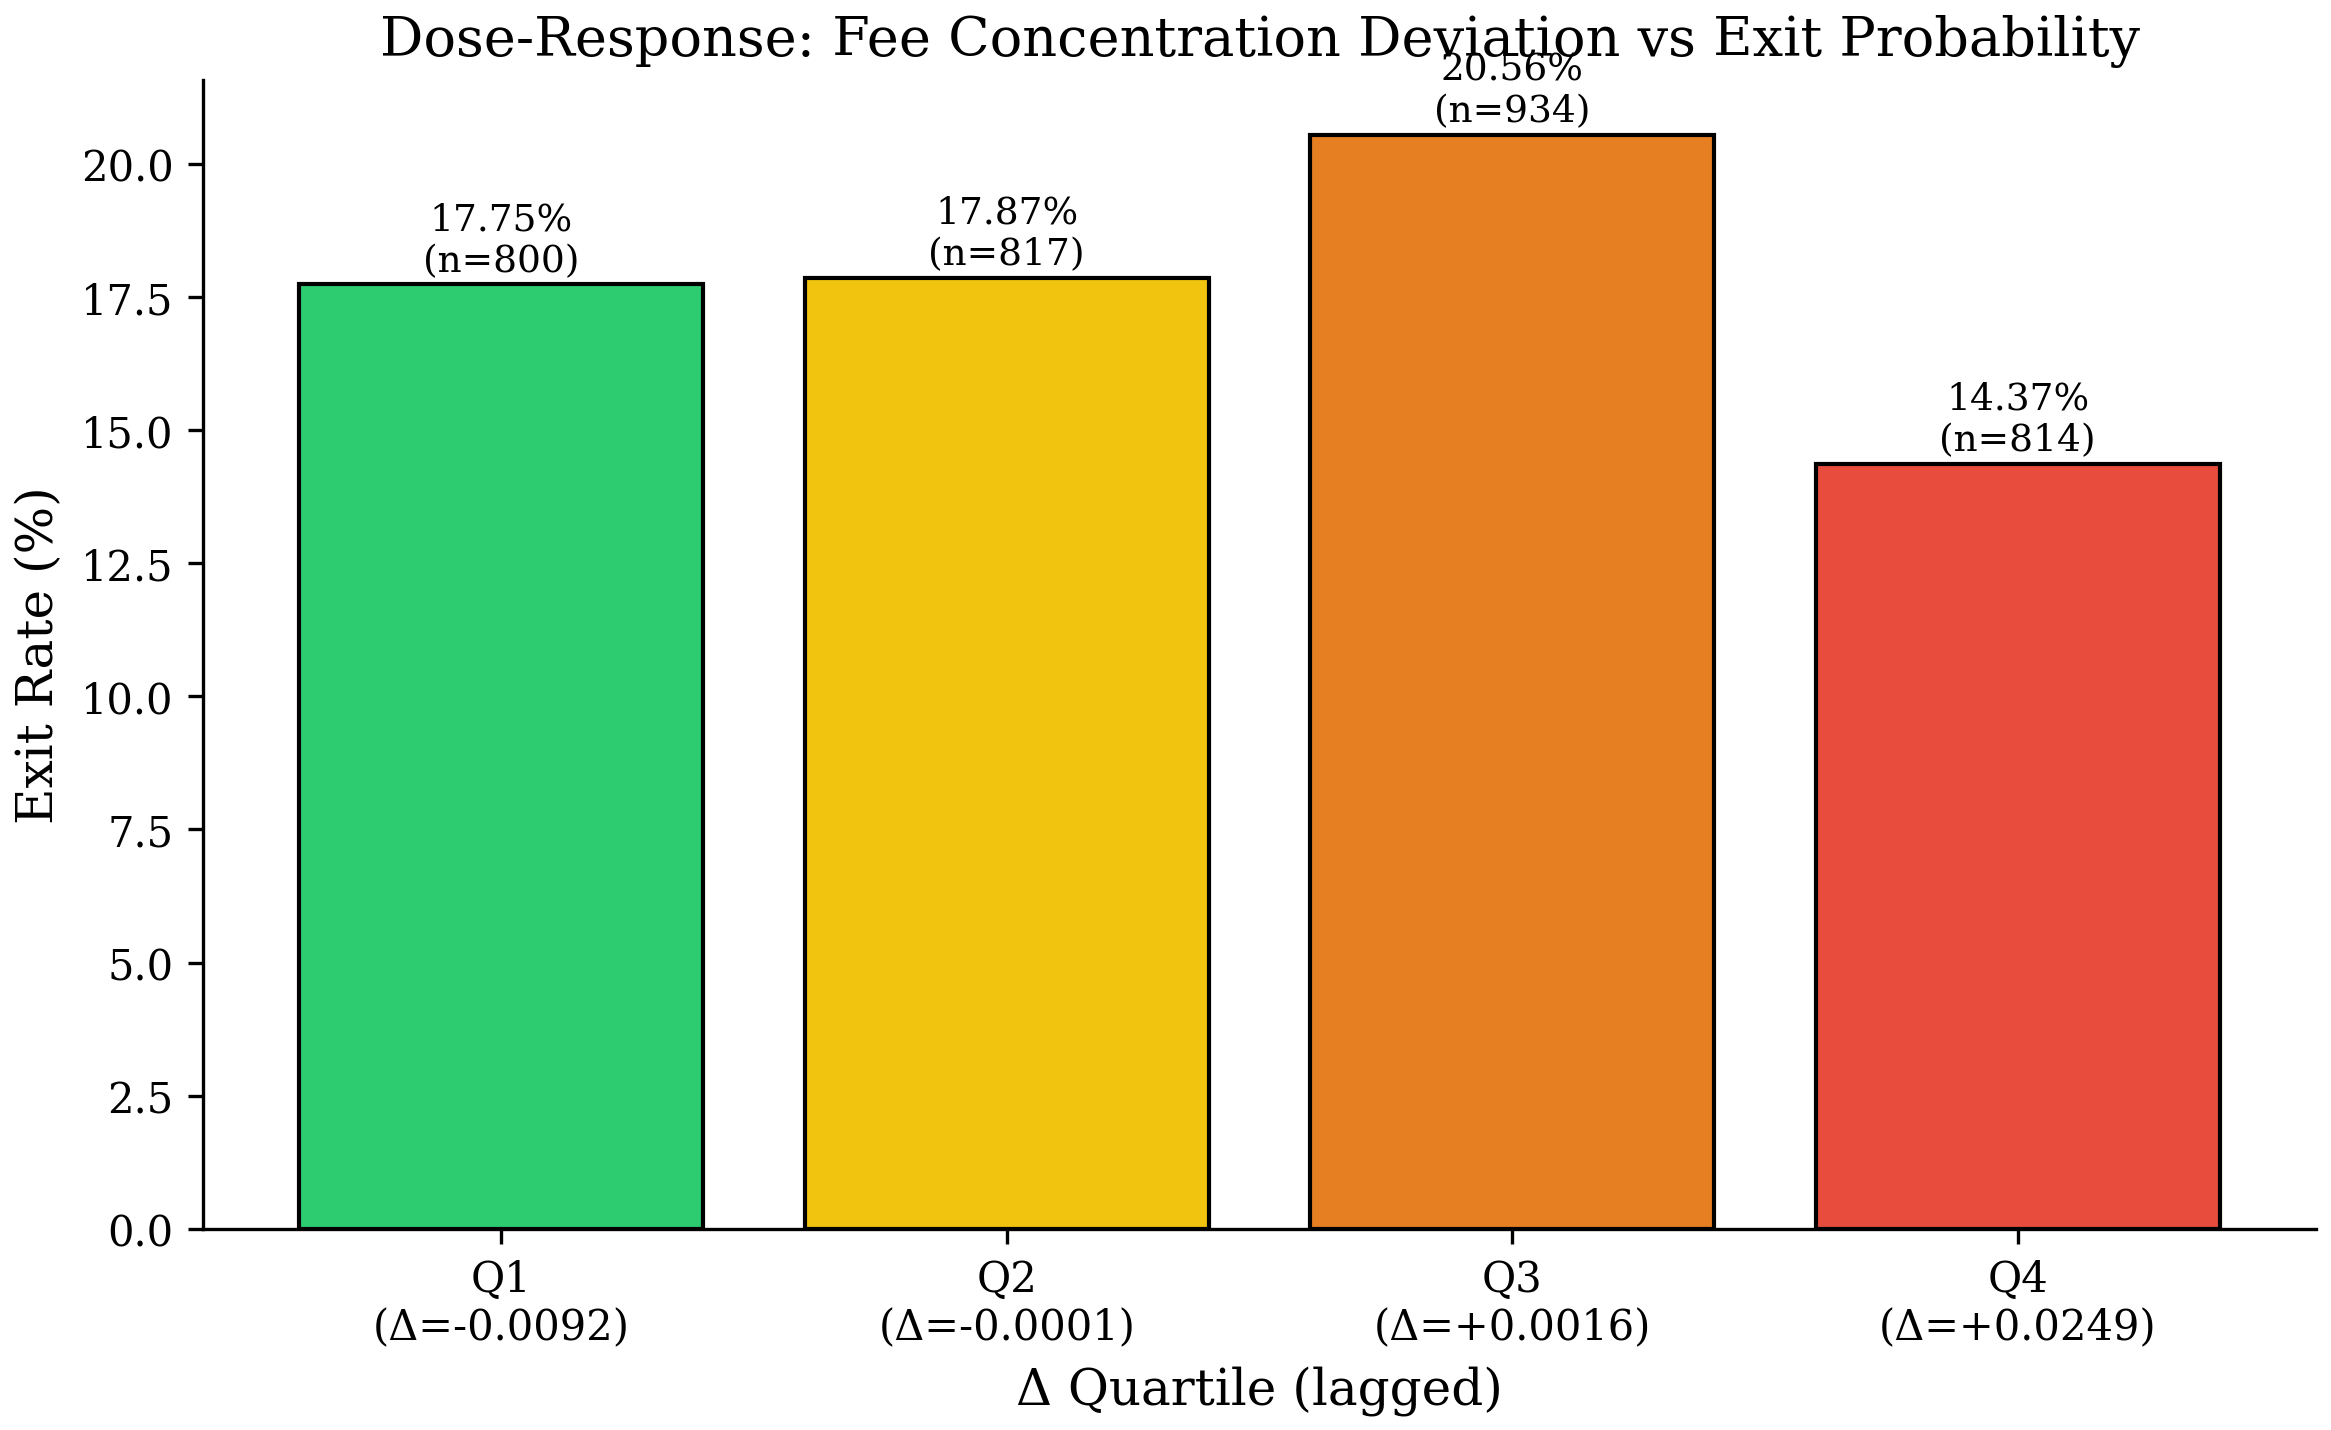
\includegraphics[width=\textwidth]{../figures/dose-response.png}
\end{center}
\end{column}

\end{columns}

\end{frame}

% --- Solution, Demo, Roadmap frames in Plan 02 ---
